\chapter{Iteration 1 (FYP-1 Mid)}
\label{ch:iter1}
\begin{itemize}
    \item FYP 1 Mid: 
    \begin{itemize}
    \item Literature review related Metaverse, and Healthcare
    \item Designed Use-case, System Diagram
    \end{itemize}
\end{itemize}


\section{Literature review related Metaverse, and Healthcare}
{This literature review explores the potential of metaversion in healthcare, a virtual, interconnected digital realm. It examines current research, technology, and developments in metaversion, focusing on historical perspectives, technological foundations, practical applications, ethical considerations, and future prospects. The review aims to illuminate the current state of knowledge and pave the way for further advancements in this rapidly evolving field.
}

\section{Designed Use-case, System Diagram}
\begin{itemize}
    \item Use Case 
    \item System Diagram
    \item Activity Diagram
\end{itemize}


\section{Use Case Diagram}
A use case diagram visualizes main system activities and interactions, identifying main processes in ovals. It is drawn from a scenario to explain system functioning.
\begin{figure}[h]
    \centering
    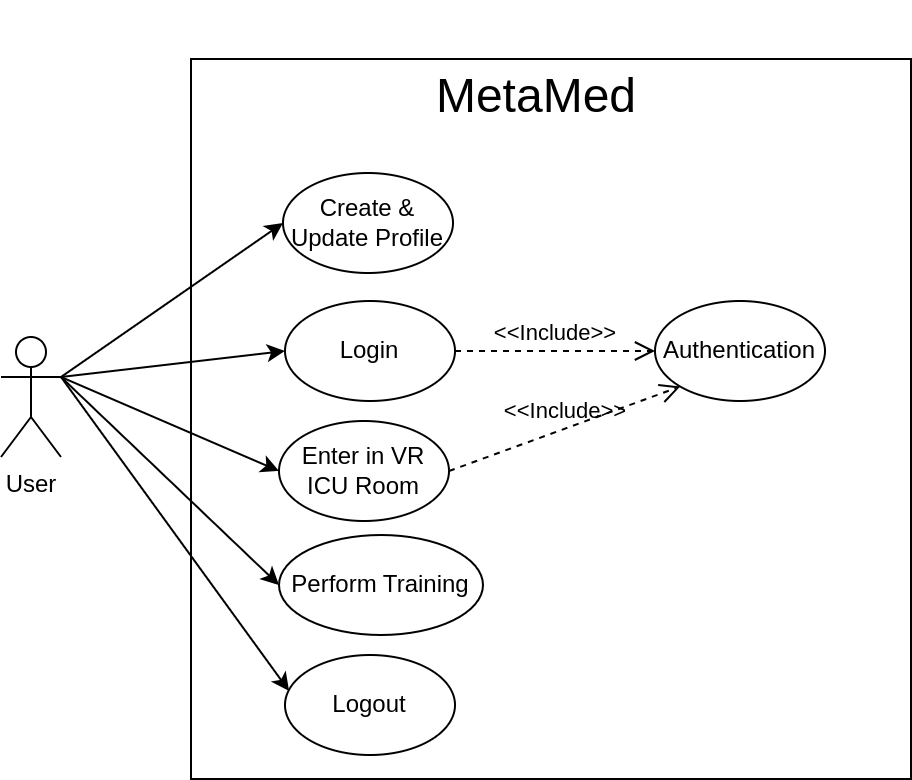
\includegraphics[width=0.5\textwidth, height=0.3\textheight]{Images/Use Case.drawio.png}
    \caption{Use Case Diagram}
    \label{fig:system-diagram}
\end{figure}

\section{System Diagram}
System Diagrams are visual representations of dynamic forces and interactions within a process, serving as more than just a process flow chart.
\begin{figure}[h]
    \centering
    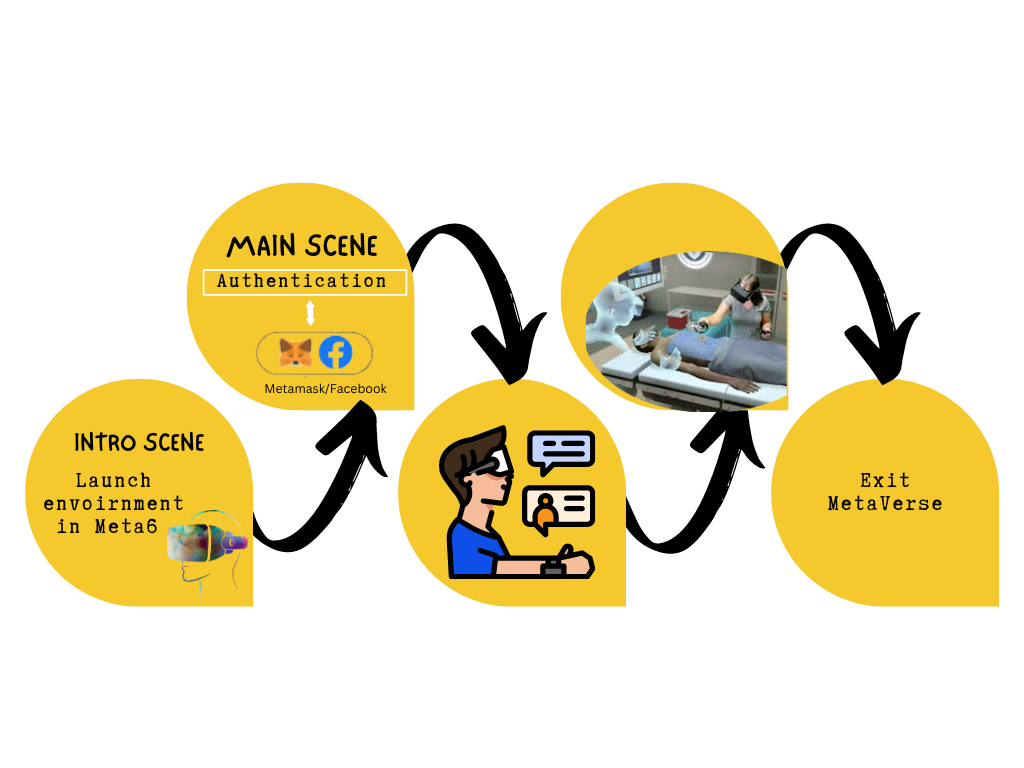
\includegraphics[width=0.7\textwidth, height=0.3\textheight]{Images/system.png}
    \caption{System Diagram}
    \label{fig:system-diagram}
\end{figure}


\section{Activity Diagram}
Activity diagrams are visual representations of a system's behavior, used to model various systems and processes, including business workflows, software systems, and organizational processes.
\begin{figure}[h]
    \centering
    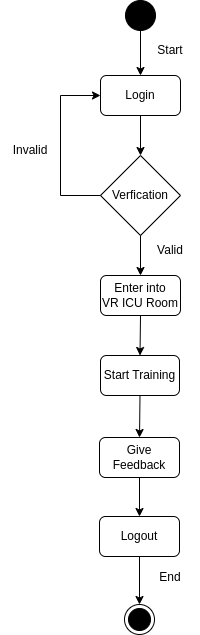
\includegraphics[width=0.3\textwidth, height=0.6\textheight]{Images/Activity.drawio.png}
    \caption{Activity Diagram}
    \label{fig:system-diagram}
\end{figure}